% ANTTHING FROM 15.2 (general regions)

% 15.2
% LOGARITHM AND EXPONENTIALS
\ifnum \Version=1
    \part $\displaystyle \int_1^{e}\int_{\ln(x)}^{1} \, dy \, dx = \int_a^b \int_c^d dx \, dy$ where $a=\framebox{\strut\hspace{0.8cm}}$, $b=\framebox{\strut\hspace{0.8cm}}$, $c=\framebox{\strut\hspace{0.8cm}}$, $d=\framebox{\strut\hspace{0.8cm}}$.
    
    \ifnum \Solutions=1 
    {\color{DarkBlue} Changing the order of integration $\displaystyle 
        \int_1^{e}\int_{\ln(x)}^{1} f(x,y) \, dy \, dx
         \ = \int_0^{1}\int_{1}^{e^y} f(x,y) dx dy $.
         }
   \else

   \fi
\fi 


% 15.2
% TRIANGULAR REGION, TWO INTEGRALS TO ONE
\ifnum \Version=2
    \part $\displaystyle \int_{-1}^{2} \int_{-x}^{1} f(x,y) d y \, d x + \int_{2}^{5} \int_{x-4}^{1} f(x,y) d y \, d x = \int_{a}^{b} \int_{c}^{d} f(x,y) \, d x\,  d y$, where 
    $a=\framebox{\strut\hspace{0.8cm}}$, $b=\framebox{\strut\hspace{0.8cm}}$, $c=\framebox{\strut\hspace{0.8cm}}$, and $d=\framebox{\strut\hspace{0.8cm}}$.    

    \ifnum \Solutions=1 
    {\color{DarkBlue}
    We are given two regions: 
    \begin{align}
        R_1: &\ -1 \le x \le 2, \quad -x \le y \le 1 \\
        R_2: &\ 2 \le x \le 5, \quad x-4 \le y \le 1
    \end{align}
    The region is also
    \begin{align}
            -y \le x \le y+4, \quad -2 \le y \le 1
    \end{align}
    Thus
    \begin{align}
        V = \int_{-2}^1\int_{-y}^{y+4} f(x,y) \, dx\, dy
    \end{align}
    }
   \else

   \fi
\fi 


% 15.2
% TRIANGULAR REGION ONE DOUBLE TO ONE DOUBLE
\ifnum \Version=3
    \part $\displaystyle \int_0^2\int_x^2 \, dy\, dx = \int_a^b\int_c^d \, dx\, dy$, where $a=\framebox{\strut\hspace{0.8cm}}$, $b=\framebox{\strut\hspace{0.8cm}}$, $c=\framebox{\strut\hspace{0.8cm}}$, and $d=\framebox{\strut\hspace{0.8cm}}$.
    
    \ifnum \Solutions=1 
    {\color{DarkBlue}
    We are given that 
    \begin{align}
        0 \le x \le 2, \quad x \le y \le 2
    \end{align}
    The region is also
    \begin{align}
        0 \le x \le y, \quad 0 \le y \le 2
    \end{align}
    Thus
    \begin{align}
        \displaystyle \int_0^2\int_x^2 \, dy\, dx = \int_0^2\int_0^y \, dx\, dy
    \end{align}
    So
    \begin{align}
        a &= 0 \\
        b &= 2 \\
        c &= 0 \\
        d &= y
    \end{align}
    }
   \else

   \fi
\fi 


% 15.2
% REGION ABOVE A PARABOLA
\ifnum \Version=4
    \part $\displaystyle \int_{0}^{1} \int_{x^2}^{1}  d y \, d x = \int_{a}^{b} \int_{c}^{d}  d x\,  d y$, where 
    $a=\framebox{\strut\hspace{0.8cm}}$, $b=\framebox{\strut\hspace{0.8cm}}$, $c=\framebox{\strut\hspace{0.8cm}}$, and $d=\framebox{\strut\hspace{0.8cm}}$.    

    \ifnum \Solutions=1 
    {\color{DarkBlue}
    We are given that 
    \begin{align}
        0 \le x \le 1, \quad x^2 \le y \le 1
    \end{align}
    The region is also
    \begin{align}
        0 \le x \le \sqrt y, \quad 0 \le y \le 1
    \end{align}
    Thus
    \begin{align}
        \int_{0}^{1} \int_{x^2}^{1}  d y \, d x = \int_0^1\int_0^{\sqrt y} \, dx\, dy
    \end{align}
    So
    \begin{align}
        a &= 0 \\
        b &= 1 \\
        c &= 0 \\
        d &= \sqrt y
    \end{align}    
    }
   \else

   \fi
\fi 



% REGION OUTSIDE CIRCLE
\ifnum \Version=5
    \part $\displaystyle \int_{0}^{2} \int_{\sqrt{4-x^2}}^{2}  dy \, dx = \int_{a}^{b} \int_{c}^{d}  d x\,  d y$, where 
    $a=\framebox{\strut\hspace{0.8cm}}$, $b=\framebox{\strut\hspace{0.8cm}}$, $c=\framebox{\strut\hspace{0.8cm}}$, and $d=\framebox{\strut\hspace{0.8cm}}$.    

    \ifnum \Solutions=1 
    {\color{DarkBlue}
    We are given that 
    \begin{align}
        0 \le x \le 2, \quad \sqrt{4 - x^2} \le y \le 2
    \end{align}
    The region is also
    \begin{align}
        0 \le y \le 2, \quad \sqrt{4 - y^2} \le x \le 2
    \end{align}
    Thus
    \begin{align}
        \int_{0}^{2} \int_{\sqrt{4-x^2}}^{2}  d y \, d x = \int_0^2\int_{\sqrt{4 - y^2}}^2 \, dx \, dy
    \end{align}
    So
    \begin{align}
        a &= 0 \\
        b &= 2 \\
        c &= \sqrt{4-y^2} \\
        d &= 2
    \end{align}    
    }
   \else

   \fi
\fi 




% 15.2
% TRIANGULAR REGION, TWO INTEGRALS TO ONE
\ifnum \Version=6
    \part $\displaystyle \int_{-3}^{1} \int_{-x}^{3} f(x,y) d y \, d x + \int_{1}^{5} \int_{x-2}^{3} f(x,y) d y \, d x = \int_{a}^{b} \int_{c}^{d} f(x,y) \, d x\,  d y$, where 
    $a=\framebox{\strut\hspace{1.4cm}}$, $b=\framebox{\strut\hspace{1.4cm}}$, $c=\framebox{\strut\hspace{3cm}}$, and $d=\framebox{\strut\hspace{3cm}}$.    

    \ifnum \Solutions=1 
    {\color{DarkBlue}
    We are given two regions: 
    \begin{align}
        R_1: &\ -3 \le x \le 1, \quad -x \le y \le 3 \\
        R_2: &\ 1 \le x \le 5, \quad x-2 \le y \le 3
    \end{align}
    It can help to sketch the region, as shown in the diagram below. 
       \begin{center}     
        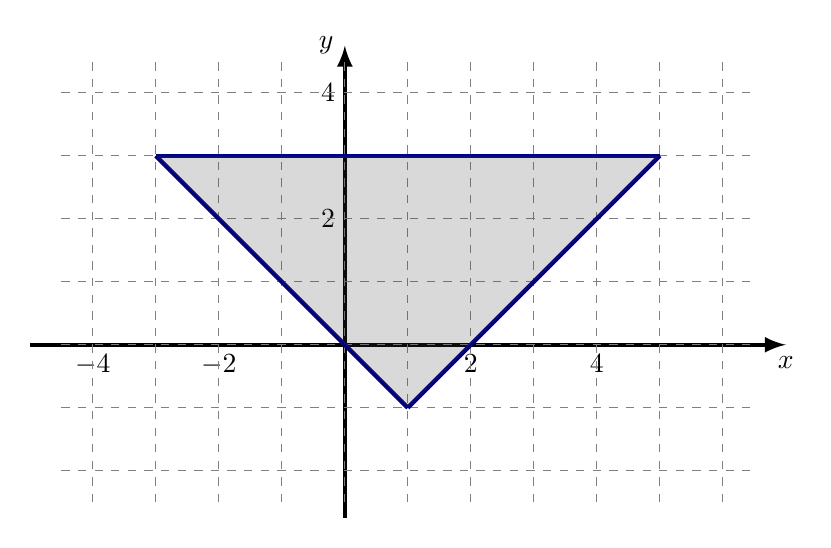
\begin{tikzpicture}[scale=0.8]
        \draw[ultra thick,->,>=latex] (-5,0)--(7,0) node[below] {$x$};
        \draw[ultra thick,->,>=latex] (0,-2.75)--(0,4.75) node[left] {$y$};
        \draw (-4,0) node[below] {$-4$};          
        \draw (-2,0) node[below] {$-2$};          
        \draw (2,0) node[below] {$2$};          
        \draw (4,0) node[below] {$4$};          
        \draw (0,2) node[left] {$2$};        
        \draw (0,4) node[left] {$4$};
        \draw[help lines,gray,thin,dashed] (-4.5, -2.5) grid (6.5, 4.5);
        \draw[domain=-3:1,ultra thick,DarkBlue,samples=4] plot ({\x},{-\x });
        \draw[domain=1:5,ultra thick,DarkBlue,samples=4] plot ({\x},{\x-2});
        \draw[ultra thick,-,DarkBlue,>=latex] (-3,3)--(5,3);
        \draw[fill=gray!50!black, opacity=0.2] (-3,3) -- (1,-1) -- (5,3);                
    \end{tikzpicture}
    \end{center}      
    The region is also
    \begin{align}
            -y \le x \le y+2, \quad -1 \le y \le 3
    \end{align}
    Thus
    \begin{align}
        V = \int_{-1}^3\int_{-y}^{y+2} f(x,y) \, dx\, dy
    \end{align}
    }
   \else
   \fi
\fi 

% REGION OUTSIDE CIRCLE
\ifnum \Version=7
    \part $\displaystyle \int_{0}^{4} \int_{\sqrt{16-x^2}}^{4}  dy \, dx = \int_{a}^{b} \int_{c}^{d}  d x\,  d y$, where 
    $a=\framebox{\strut\hspace{1cm}}$, $b=\framebox{\strut\hspace{1cm}}$, $c=\framebox{\strut\hspace{2cm}}$, and $d=\framebox{\strut\hspace{2cm}}$.    

    \ifnum \Solutions=1 
    {\color{DarkBlue}
    We are given that 
    \begin{align}
        0 \le x \le 4, \quad \sqrt{16 - x^2} \le y \le 4
    \end{align}
    The region is also
    \begin{align}
        0 \le y \le 4, \quad \sqrt{16 - y^2} \le x \le 4
    \end{align}
    Thus
    \begin{align}
        \int_{0}^{4} \int_{\sqrt{16-x^2}}^{4}  d y \, d x = \int_0^4\int_{\sqrt{16 - y^2}}^4 \, dx \, dy
    \end{align}
    So
    \begin{align}
        a &= 0 \\
        b &= 4 \\
        c &= \sqrt{16-y^2} \\
        d &= 4
    \end{align}    
    }
   \else

   \fi
\fi 







% 15.2
% WEIRD REGION, TWO INTEGRALS TO ONE, MAYBE A HARD QUESTION? 
\ifnum \Version=8
    \part $\displaystyle \int_{1}^{5} \int_{0}^{\sqrt{x-1}} f(x,y) d y \, d x + \int_{5}^{7} \int_{0}^{7-x} f(x,y) d y \, d x = \int_{a}^{b} \int_{c}^{d} f(x,y) \, d x\,  d y$, where 
    $a=\framebox{\strut\hspace{1.5cm}}$, $b=\framebox{\strut\hspace{1.5cm}}$, $c=\framebox{\strut\hspace{4cm}}$, and $d=\framebox{\strut\hspace{4cm}}$.    

    \ifnum \Solutions=1 
    {\color{DarkBlue}
    We are given two regions: 
    \begin{align}
        R_1: &\ 1 \le x \le 5, \quad 0 \le y \le \sqrt{x-1} \\
        R_2: &\ 5 \le x \le 7, \quad 0 \le y \le \sqrt{7-x}
    \end{align}
    The region is also
    \begin{align}
            y^2+1 \le x \le 7-x, \quad 0 \le y \le 2
    \end{align}
    Thus
    \begin{align}
        a &= 0 \\
        b &= 2 \\
        c &= y^2+1 \\
        d &= 7-x
    \end{align}
    }
   \else
   \fi
\fi 




% 15.2
% REGION ABOVE A PARABOLA
\ifnum \Version=9
    \part Let $\displaystyle A = \iint_R  d y \, d x = \int_{a}^{b} \int_{c}^{d}  d x\,  d y$, where $R=\{(x,y) \in \mathbb R^2 \, | \,0 \le x \le 2, \ x^2+1 \le y \le 5 \} $. Then 
    $a=\framebox{\strut\hspace{1.5cm}}$, $b=\framebox{\strut\hspace{1.5cm}}$, $c=\framebox{\strut\hspace{2cm}}$, and $d=\framebox{\strut\hspace{3cm}}$.    

    \ifnum \Solutions=1 
    {\color{DarkBlue}
    We are given that 
    \begin{align}
        0 \le x \le 2, \quad x^2+1 \le y \le 5
    \end{align}
    The region is also
    \begin{align}
        0 \le x \le \sqrt {y-1}, \quad 1 \le y \le 5
    \end{align}
    Thus
    \begin{align}
        \int_{0}^{2} \int_{x^2+1}^{1}  d y \, d x = \int_1^5\int_0^{\sqrt{y-1}} \, dx\, dy
    \end{align}
    So
    \begin{align}
        a &= 1\\
        b &= 5 \\
        c &= 0 \\
        d &= \sqrt{y-1}
    \end{align}    
    }
   \else

   \fi
\fi 
